\documentclass[../../main.tex]{subfiles}
\begin{document}


\begin{problem}
给定一个带期限的作业排序问题($n = 5$):
\begin{align*}
     & (p_1, p_2, p_3, p_4, p_5) = (6, 3, 4, 8, 5), \\
     & (t_1, t_2, t_3, t_4, t_5) = (2, 1, 2, 1, 1), \\
     & (d_1, d_2, d_3, d_4, d_5) = (3, 1, 4, 2, 4).
\end{align*}


\begin{enumerate}
    \item 应用 \texttt{FIFOBB} 求使总罚款数最小的可行作业集 $J$,求出对应于最优解的罚款值,并画出状态空间树(采用大小可变的元组).

    \item 应用 \texttt{LCBB} 求使总罚款数最小的可行作业集 $J$,求出对应于最优解的罚款值,并画出状态空间树(采用大小固定的元组).
\end{enumerate}
\end{problem}

\begin{solution}
\end{solution}
1. 应用 \texttt{FIFOBB}
\begin{center}
    \begin{tikzpicture}[scale=0.5]
        \tikzset{every tree node/.style={ draw, rectangle}}
        \Tree
        [.\(1:\hat{c}=0,u=26\)
            [.\(2:\hat{c}=0,u=20\)
                    [.\(7:\hat{c}=0,u=17\) [.\(17:-\) ] [.\(18:-\) ] [.\(19:\hat{c}=15,u=15\) ]]
                        [.\(8:\hat{c}=3,u=16\) [.\(20:-\) ] [.\(21:-\) ] ]
                        [.\(9:\hat{c}=7,u=12\) [.\(22:\hat{c}=7,u=7\) ]]
                        [.\(10:\hat{c}=15,u=15\) ]
                ]
                [.\(3:\hat{c}=6,u=23\)
                    [.\(11:\hat{c}=6,u=19\) [.\(23:\hat{c}=11>7\) ][.\(24:\hat{c}=14>7\) ]] [.\(12:\hat{c}=10,u=15\) [.\(25:\hat{c}=10>7\) ]] [.\(13:\hat{c}=18>15\) ]
                ]
                [.\(4:\hat{c}=9,u=22\)
                    [.\(14:\hat{c}=9,u=14\) [.\(26:\hat{c}=9>7\) ]] [.\(15:\hat{c}=17>14\) ]
                ]
                [.\(5:\hat{c}=13,u=18\)
                    [.\(16:\hat{c}=13,u=13\) ]
                ]
                [.\(6:\hat{c}=21>18\) ]
        ]
    \end{tikzpicture}
\end{center}
其中22号节点的\(\hat{c}\)最小, 因此是最优解: \(J = \{1,4,5\}\), 罚款值为7.


2. 应用 \texttt{LCBB}
\begin{center}
    \begin{tikzpicture}[scale=0.55]
        \tikzset{every tree node/.style={ draw, rectangle}}
        \Tree
        [.\(1:\hat{c}=0,u=26\)
            [.\(2:\hat{c}=0,u=20\)
                    [.\(4:\hat{c}=0,u=17\)
                            [.\(6:\hat{c}=0,u=13\) [.\(8:-\) ]]
                                [.\(7:\hat{c}=4,u=17\)
                                    [.\(15:-\) ] [.\(16:\hat{c}=12>8\) ]
                                ]
                        ]
                        [.\(5:\hat{c}=3,u=20\)
                            [.\(9:\hat{c}=3,u=16\)
                                    [.\(11:\hat{c}=3,u=8\) [.\(13:-\) ] [.\(14:\hat{c}=8,u=8\) ]] [.\(12:\hat{c}=11,u=16\) [.\(29:-\) ] [.\(30:\hat{c}=11>8\) ]]
                                ] [.\(10:\hat{c}=7,u=20\) [.\(19:\hat{c}=7,u=12\) [.\(21:\hat{c}=7,u=7\) ] [.\(22:\hat{c}=12>8\) ]] [.\(20:\hat{c}=15>8\) ]]
                        ]
                ]
                [.\(3:\hat{c}=6,u=23\)
                    [.\(17:\hat{c}=6,u=23\) [.\(23:\hat{c}=6,u=19\) [.\(25:\hat{c}=6,u=11\) [.\(27:-\) ] [.\(28:\hat{c}=11>8\) ]] [.\(26:\hat{c}=14>8\) ]][.\(24:\hat{c}=10>8\) ]]
                        [.\(18:\hat{c}=9>8\) ]
                ]
        ]
    \end{tikzpicture}
\end{center}
其中21号节点的\(\hat{c}\)最小, 因此是最优解: \(J = \{1,4,5\}\), 罚款值为7.

\end{document}